\documentclass[10pt,CJKmath]{zhbook-v1}
%\xeCJKsetup{CJKmath=true}
\usepackage{tikz}
\usetikzlibrary{arrows.meta,shapes.geometric,positioning,shadows,fit,backgrounds}
% Global TikZ styles for consistent, polished diagrams
\tikzset{
  base/.style={font=\small, align=center,inner sep=2pt,outer sep=0mm},
  block/.style={rectangle, draw=black!60, rounded corners, minimum width=20mm, minimum height=8mm, align=center, fill=teal!6, drop shadow, base},
  proc/.style={rectangle, draw=black!60, minimum width=38mm, minimum height=8mm, align=center, fill=orange!6, drop shadow, base},
  box/.style={rectangle, draw=black!45, rounded corners, minimum width=40mm, minimum height=8mm, align=center, fill=gray!6, base},
  arrow/.style={-{Latex[length=3mm]}, very thick, line cap=round, color=black!70}
}

\usepackage{fontawesome5}
\setmintedinline[c++]{breaklines,breakanywhere,bgcolor=none,breakanywheresymbolpre=\rotatebox{-90}{\mbox{\tiny\textcolor{pink}{\faLevelDown*}}}}
\newcommand{\il}[1]{\mintinline{c++}{#1}}%

\newtcbox{\mybox}[1][red]{on line,colupper=black,fonttitle=\bfseries,
 arc=4pt,outer arc=4pt,colback=yellow!10!white,colframe=#1!50!black,
 boxsep=0pt,left=2pt,right=2pt,top=1pt,bottom=1pt,
 boxrule=1pt,leftrule=1pt,rightrule=1pt}
 
 
\begin{document}
		%\frontmatter
    %\tableofcontents

\mainmatter
\pagestyle{fancy}
\setchapterimage{./images/background}

\chapter{启始}
\section{项目设置}

本节介绍如何从头创建并配置一个用于实现角色移动(locomotion)的 Unreal Engine 项目。主要要点如下:

首先确保已安装 Unreal Engine(建议使用 5.3 及以上版本,作者示例使用 5.6.x),可通过 Epic Games Launcher 的 Unreal Engines 库安装合适版本。创建项目时选择“Blank”模板、Blueprint 项目类型,并按需设置平台(如 Desktop)与品质预设。

创建后:
\begin{itemize}
\item 在插件(Edit \faArrowAltCircleRight Plugins)中禁用(\il{Modeling Tools Editor Mode}、\il{Open Image Denoise})等不需要的插件,以减少体积与复杂度,并重启引擎。
\item 下载并迁移作者提供的启动内容包(LS Essentials):该包包含必要的模型、动画、网格、占位材质与原型关卡资源。迁移时确保目标是新项目的 Content 目录,并注意版本兼容(LS Essentials 为 5.3,目标项目应 ≥5.3)。
\end{itemize}
工程组织建议:
\begin{itemize}
\item 在 Content 下建立专用目录(例如\il{LocomotionSystem})并在开发阶段保留一个独立的 \il{LS_Essentials} 源内容文件夹,便于日后更新与再迁移;最终可将稳定资源合并到主目录。
\item 在 $Maps \rightarrow Showcase$ 下创建一个简化的测试关卡(如 \il{map_showcase})用于快速迭代与调试。
\end{itemize}
创建基础蓝图类(存放于 \mybox{Blueprints/GameBase}):
\begin{itemize}
\item  GameMode(命名示例:\il{BP_LocomotionSystem_GM})
\item  PlayerController(\il{BP_LocomotionSystem_PC})用于处理玩家输入与控制逻辑
\item  HUD(`\il{BP_LocomotionSystem_HUD}`)用于将来显示血条、调试信息等 UI 元素
\end{itemize}
在 GameMode 中绑定自定义的 PlayerController 与 HUD,并在 $Project Settings \rightarrow Maps \& Modes$ 中将默认地图与默认 GameMode 设置为刚创建的 \il{map_showcase} 与 \il{BP_LocomotionSystem_GM}。保存并编译项目。

当前状态:运行时显示为观众相机(spectator),尚未添加可控制的角色;下一步将是导入/创建角色并实现移动与动画系统的集成。

\section{添加角色模型与摄像机}

本节演示如何在项目中添加角色蓝图、组织角色文件夹、将骨骼网格(skeletal mesh)连接到角色并为玩家角色配置摄像机。要点和步骤如下:

\begin{enumerate}
  \item 目标与目录结构
    \begin{itemize}
      \item 目标:在关卡中放置可见的角色实例(替代默认的观众摄像机 spectator camera)。
      \item 建议在 Content 下创建目录 \il{LocomotionSystem},并在其中创建 \il{Characters} 文件夹;在 \il{Characters} 内再创建 \il{Blueprints} 用于存放角色蓝图。
    \end{itemize}

  \item 使用 \il{Character} 类与继承设计
    \begin{itemize}
      \item 使用 Unreal 的 \il{Character} 蓝图类(而非通用 \il{Actor}),因为 \il{Character} 内置移动控制(movement)相关功能更便捷。
      \item 创建一个父级蓝图:\il{BP_CharacterBase},作为通用父类,包含所有角色共享特性(例如胶囊体、箭头、通用组件与默认配置)。
      \item 从父类派生子类以区分玩家与 NPC:
        \begin{itemize}
          \item \il{BP_PlayerBase} — 供玩家控制的角色(在 GameMode 中设为默认出生类)。
          \item \il{BP_NPCBase} — 供 AI 控制的非玩家角色。
        \end{itemize}
      \item 采用面向对象继承:所有常见修改应在父类(\il{BP_CharacterBase})中进行,以便子类自动继承,避免在子类重复修改带来的维护问题。
    \end{itemize}

  \item 组织资源与文件夹
    \begin{itemize}
      \item 按功能创建子文件夹:例如 \il{Base}(放 \il{BP_CharacterBase})、\il{Player}(放 \il{BP_PlayerBase})、\il{NPC}(放 \il{BP_NPCBase}),以便后续扩展管理多个实例。
    \end{itemize}

  \item 添加并配置骨骼网格(Skeletal Mesh)
    \begin{itemize}
      \item 从启动内容包 \il{LS_Essentials}(路径示例:\il{Characters/Mannequins} 下的 \il{Meshes})中挑选合适的骨骼网格(例如来自第三人称模板的骨骼网格)。
      \item 在父类或合适的蓝图组件中将该骨骼网格设为 Mesh 组件(推荐放在 \il{BP_CharacterBase}),然后调整位置与朝向(例如位置和旋转可能需分别修正为 -90° 等),确保模型面向箭头组件方向。
      \item 注意:不要仅在子类(例如直接在 \il{BP_PlayerBase})修改骨骼网格的通用变换,否则这些修改不会回写到父类;最佳做法是在父类中完成通用变换。
    \end{itemize}

  \item 将玩家蓝图设为默认生成类与常见问题
    \begin{itemize}
      \item 在 GameMode 或 Project Settings → Maps \& Modes 中,将默认生成(Default Pawn / Default Pawn Class)设置为 \il{BP_PlayerBase}。
      \item 初次运行后可能出现的问题:
        \begin{itemize}
          \item 无法控制角色(角色可见但无响应):通常是因为尚未将摄像机或控制逻辑添加到玩家蓝图 \il{BP_PlayerBase}。
          \item 出现奇怪的网格:可能是角色已被放置但摄像机仍为观众摄像机,或摄像机未绑定到玩家蓝图。
        \end{itemize}
    \end{itemize}

  \item 为玩家添加摄像机与弹簧臂(Spring Arm)
    \begin{itemize}
      \item 仅在 \il{BP_PlayerBase} 中添加摄像机与 \il{SpringArm}(不要在 \il{BP_CharacterBase} 或 \il{BP_NPCBase} 中添加摄像机——摄像机只用于玩家控制)。
      \item 在 \il{CapsuleComponent} 下添加一个 \il{SpringArm} 组件,再将 \il{Camera} 设为其子组件。\il{SpringArm} 提供相对位移(例如默认 X 轴偏移约 300 或 400 单位),通过调整长度可以控制摄像机远近(示例:400 为合适初始值)。
      \item \il{SpringArm} 的好处:便于管理相机与角色间的固定距离,并在碰撞时处理镜头回缩。
    \end{itemize}

  \item 编译、保存与测试
    \begin{itemize}
      \item 在对蓝图进行修改后,编译并保存蓝图,然后运行测试(Play)。
      \item 运行时:如果摄像机与控制逻辑未添加,角色(例如 \il{BP_PlayerBase})虽然可见但不可控制;完成摄像机与后续控制逻辑(下一节)后即可控制移动。
    \end{itemize}

  \item 下一步
    \begin{itemize}
      \item 在下一节教程中添加玩家输入与控制逻辑(绑定输入、实现移动与转向逻辑),并将这些控制逻辑集成到 \il{BP_PlayerBase} 中。
    \end{itemize}
\end{enumerate}

\section{增强输入系统与摄像机控制(含 TikZ 蓝图示意)}

本节说明如何使用增强输入系统(Enhanced Input)接收玩家输入,并将这些输入用于控制摄像机与玩家角色;同时给出对应的蓝图伪代码与 TikZ 节点示意,帮助实现 \il{IMC_Default}、\il{IA_Look} 的注册与消费。

\begin{enumerate}
  \item 简要回顾
    \begin{itemize}
      \item 创建并注册映射上下文:\il{IMC_Default}。
      \item 定义输入动作:\il{IA_Look}(类型为 Axis 2D,用于鼠标 X/Y)。
      \item 在 \il{BP_PlayerBase} 中添加摄像机相关组件(\il{SpringArm} + \il{Camera}),并在蓝图中消费 \il{IA_Look} 的输入值来驱动视角。
    \end{itemize}

  \item BeginPlay 注册流程(伪代码)

\begin{verbatim}
Event BeginPlay
  Controller := GetController()
  If Controller IsValid then
    PC := Cast(Controller, PlayerController)
    Subsystem := GetLocalPlayerSubsystem(PC)
    If Subsystem IsValid then
      Subsystem.AddMappingContext(IMC_Default, Priority=0)
\end{verbatim}

  \item BeginPlay 节点示意(TikZ 图)
  \begin{center}
  \begin{tikzpicture}[node distance=10mm and 20mm, every node/.style={font=\small}]
    \tikzset{block/.style={rectangle, draw, rounded corners, minimum width=28mm, minimum height=7mm, align=center, fill=white}}
    \tikzset{arrow/.style={-{Latex[length=3mm]}, thick}}

    \node[block] (begin) {Event BeginPlay};
    \node[block, below=of begin] (getc) {Get Controller};
    \node[block, below=of getc] (cast) {Cast to PlayerController};
    \node[block, below=of cast] (subsys) {Get Local Player Subsystem (Enhanced Input)};
    \node[block, below=of subsys] (add) {Add Mapping Context\newline(\il{IMC_Default}, Priority=0)};

    \draw[arrow] (begin) -- (getc);
    \draw[arrow] (getc) -- (cast);
    \draw[arrow] (cast) -- (subsys);
    \draw[arrow] (subsys) -- (add);
  \end{tikzpicture}
  \end{center}

  \item 绑定并消费 \il{IA_Look}(伪代码)
\begin{verbatim}
// 在 BP_PlayerBase 的 Event Graph 中添加 Enhanced Input Action 事件
OnInputAction(IA_Look)  // triggered with Axis2D value (X, Y)
  (X, Y) := BreakAxis2D(InputValue)
  // 加入灵敏度与可选反转
  AddControllerYawInput( X * Sensitivity )   // 水平(偏航)
  AddControllerPitchInput( Y * Sensitivity ) // 垂直(俯仰)
\end{verbatim}

  \item IA\_Look 节点示意(TikZ 图)
  \begin{center}
  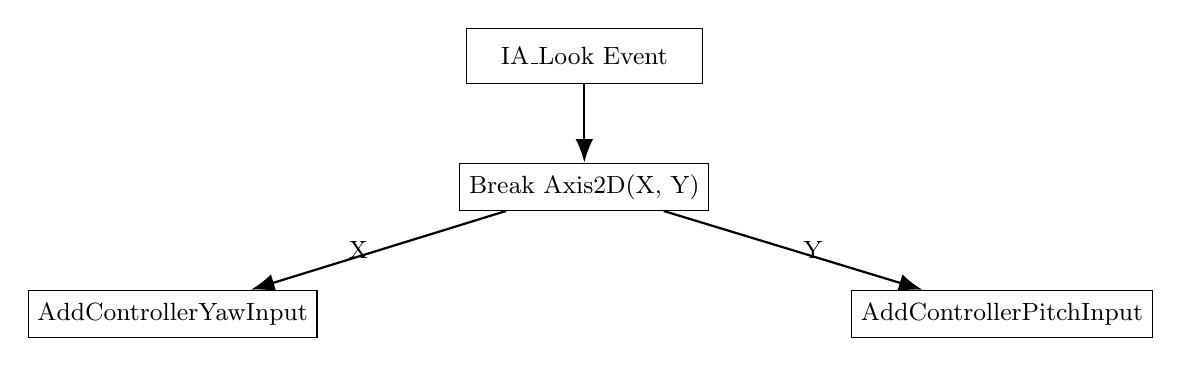
\begin{tikzpicture}[node distance=10mm and 18mm, every node/.style={font=\small}]
    \tikzset{proc/.style={rectangle, draw, minimum width=30mm, minimum height=7mm, align=center, fill=white}}
    \tikzset{small/.style={rectangle, draw, minimum width=22mm, minimum height=6mm, align=center, fill=white}}
    \tikzset{arrow/.style={-{Latex[length=3mm]}, thick}}

    \node[proc] (event) {IA\_Look Event};
    \node[small, below=of event] (break) {Break Axis2D \newline (X, Y)};
    \node[small, below left=of break] (yaw) {AddControllerYawInput};
    \node[small, below right=of break] (pitch) {AddControllerPitchInput};

    \draw[arrow] (event) -- (break);
    \draw[arrow] (break) -- (yaw) node[midway, left] {X};
    \draw[arrow] (break) -- (pitch) node[midway, right] {Y};
  \end{tikzpicture}
  \end{center}

  \item 摄像机与弹簧臂关键设置(文本示例)
    \begin{itemize}
      \item 在 \il{BP_PlayerBase} 的 Components 中:
        \begin{itemize}
          \item CapsuleComponent(根)
          \item Mesh(Skeletal Mesh,推荐在 \il{BP_CharacterBase} 设置)
          \item SpringArm(附着在 Capsule)
            \begin{itemize}
              \item TargetArmLength := 400 (示例)
              \item bUsePawnControlRotation := true  \% 关键:允许 Pawn 的控制器旋转影响 SpringArm
            \end{itemize}
          \item Camera(附着在 SpringArm)
        \end{itemize}
      \item 若未启用 \il{bUsePawnControlRotation},则通过 AddControllerPitchInput 进行的俯仰不会反映到 Camera 上;启用后,SpringArm 会随 Pawn 的控制器旋转,Camera 会跟随显示正确俯仰/偏航。
    \end{itemize}

  \item 可选:灵敏度与反转开关(伪代码)
\begin{verbatim}
Variable Sensitivity := 1.0
Variable InvertY := true
OnInputAction(IA_Look)
  (rawX, rawY) := BreakAxis2D(InputValue)
  if InvertY then rawY := -rawY
  AddControllerYawInput(rawX * Sensitivity)
  AddControllerPitchInput(rawY * Sensitivity)
\end{verbatim}

  \item 调试技巧
    \begin{itemize}
      \item 使用 Print String 打印 X/Y 值以确认轴方向与取反行为。
      \item 若俯仰无效,检查 \il{SpringArm} 的 \il{Use Pawn Control Rotation} 是否为 true。
      \item 确认在 \il{Event BeginPlay} 中确实已为本地玩家子系统添加映射上下文(Add Mapping Context 成功)。
    \end{itemize}

  \item 插入真实蓝图截图(示例)
    \begin{verbatim}
% 若要插入真实截图,先将图片放入同一目录(或相对路径),然后在此处使用 includegraphics:
% \begin{figure}[ht]
%   \centering
%   \includegraphics[width=0.9\linewidth]{bp_ia_look_example.png}
%   \caption{在 \il{BP_PlayerBase} 中消费 \il{IA_Look} 的蓝图节点示意}
% \end{figure}
    \end{verbatim}

\end{enumerate}

\bigskip
\noindent 小结:本文件包含 BeginPlay 输入注册流程、\il{IA_Look} 的消费伪代码、以及用 TikZ 绘制的节点示意图,便于在没有编辑器截图时也能理解蓝图流程。



\section{移动控制(Movement Controls)}

本节介绍如何为玩家角色实现移动控制:创建并配置移动输入动作、在映射上下文中绑定按键、以及在蓝图中根据控制器方向将轴输入转换为世界空间的移动向量并调用移动接口。主要内容、实现步骤与示意如下。

\subsection{目标与总体思路}
使用增强输入系统(Enhanced Input)在 \il{IMC_Default} 中添加新的移动输入动作 \il{IAMove}(Axis 2D),将键盘按键(如 \il{W}, \il{A}, \il{S}, \il{D})映射为前后左右的轴值(可加 Dead Zone 与取反),然后在 \il{BP_PlayerBase} 中消费该输入,将轴值转换为基于控制器朝向的世界向量(右向量 / 前向量),并使用 \il{AddMovementInput} 以轴值为缩放因子驱动角色移动,支持组合键实现斜向移动。

\subsection{在输入映射上下文中添加移动动作}
\begin{itemize}
  \item 在项目的 \il{Inputs} → \il{Actions} 中新建输入动作:\il{IAMove}(类型:Axis 2D)。
  \item 在 \il{IMC_Default} 中加入 \il{IAMove} 的映射。
  \item 为 \il{IAMove} 绑定四个按键(按键-轴关系示例):
    \begin{description}
      \item[\il{W}] 前进(正向 y 或 forward)
      \item[\il{S}] 后退(反向:对 W 做 Negate)
      \item[\il{A}] 左移(反向:对 D 做 Negate)
      \item[\il{D}] 右移(正向)
    \end{description}
  \item 可选:为轴添加 Modifier(例如 Dead Zone),示例范围为 0.2 到 1,避免微小误差导致的漂移。
\end{itemize}

\subsection{键位绑定与 Modifier 处理}
\begin{itemize}
  \item 可以手动在键盘输入面板选择按键,或使用键选择器(点击键图标变黄并按下要绑定的键)。
  \item 对于与某按键相反的按键(例如 \il{S} 对应 \il{W}),在该按键的映射上添加 Negate Modifier,以便输入值方向正确。
  \item 对某些轴(例如左右轴)不需要对称取反则保持默认。
\end{itemize}

\subsection{在 \il{BP_PlayerBase} 中消费 \il{IAMove}(事件图与伪代码)}
在 \il{BP_PlayerBase} 的 Event Graph 中添加对 \il{IAMove} 的 Enhanced Input Action 事件,并将 Axis2D 分量映射到世界空间移动输入。关键步骤如下:

\begin{verbatim}
// 伪代码(蓝图等效)
OnInputAction(IAMove)  // Axis2D: (X, Y)
  // 水平轴 X 控制左右移动(基于控制器的 RightVector)
  ctrlRot := GetControlRotation()
  rightVector := GetRightVector(ctrlRot)   // 只取 yaw / roll as needed
  AddMovementInput(rightVector, X)

  // 垂直轴 Y 控制前后移动(基于控制器的 ForwardVector)
  forwardVector := GetForwardVector(ctrlRot) // 只取 yaw
  AddMovementInput(forwardVector, Y)
\end{verbatim}

说明:
\begin{itemize}
  \item 使用 \il{GetControlRotation} 获取控制器朝向,然后从该旋转提取 RightVector 与 ForwardVector(通常忽略 Pitch,只使用 Yaw);
  \item 将轴值作为 \il{AddMovementInput} 的 Scale 输入,从而实现速度/方向的缩放;轴值可与灵敏度变量相乘以调整响应。
  \item 若要复用节点,可复制一组以处理 X 与 Y 分量(Ctrl+C / Ctrl+V 或 Ctrl+D 快速复制节点)。
\end{itemize}

\subsection{节点/流程示意(文本版)}
\begin{enumerate}
  \item 在 \il{Event BeginPlay} 已注册 \il{IMC_Default}(此前章节)。
  \item 在事件图中添加 \il{IAMove} Input Action 事件。
  \item 使用 \il{Break Axis2D} 分解为 \il{X}, \il{Y}。
  \item 对 \il{X}:调用 \il{GetControlRotation} → 取 \il{RightVector} → \il{AddMovementInput(RightVector, X)}。
  \item 对 \il{Y}:调用 \il{GetControlRotation} → 取 \il{ForwardVector} → \il{AddMovementInput(ForwardVector, Y)}。
  \item 编译并保存,执行 Play 验证左右、前后与组合(斜向)移动。
\end{enumerate}

\subsection{调试与常见问题}
\begin{itemize}
  \item 如果左右移动有效但前后无效,确认 \il{IAMove} 的 Y 分量是否正确绑定与消费(字幕中一开始作者出现只实现 X 后才补实现 Y)。
  \item 使用 \il{Print String} 临时打印 \il{X}, \il{Y} 值以检测按键绑定与 Negate Modifier 的效果(例如 \il{S} 与 \il{A} 被 Negate 时,按下应产生负值)。
  \item 确保在计算 Forward/Right 向量时使用的是控制器的 Yaw(避免 Pitch 导致非水平向量),即可通过拆分旋转并仅使用 Yaw。
  \item Dead Zone 参数能防止手柄/摇杆微抖导致的微小移动;键盘通常不需要,但放在映射中无害。
\end{itemize}

\subsection{运行结果与用户体验}
\begin{itemize}
  \item 在完成 X(左右)与 Y(前后)的 AddMovementInput 后,玩家可使用 \il{W}/\il{A}/\il{S}/\il{D} 实现前后左右移动,并能混合输入以实现对角线移动。
  \item 即便能移动,角色的视觉表现(动画)仍处于静止或 Idle;接下来需将移动状态与动画蓝图结合(例如在下一节绑定速度参数触发走跑动画)。
\end{itemize}

\subsection{下一步建议}
\begin{itemize}
  \item 将移动状态(例如速度或 isMoving 布尔)输出到 Animation Blueprint,以在移动时播放行走/奔跑动画,在停止时播放 Idle。
  \item 为移动添加阻尼、最大速度与加速度参数,以获得更自然的加速/减速体验(可在 Character Movement 组件或手写移动逻辑中实现)。
  \item 如果使用手柄(Gamepad),为 \il{IAMove} 添加对应的摇杆轴映射,并为摇杆配置合适的 Dead Zone。
\end{itemize}



\section{动画蓝图与空闲动画(Animation Blueprint and Idle Animation)}

本节展示如何为角色分配并测试动画蓝图(Animation Blueprint),并演示将空闲(Idle)动画应用到角色骨骼网格的基本流程。下面为结构化总结与关键步骤:

\subsection{问题陈述}
当前项目已完成摄像机控制与角色移动,但在移动时角色没有播放任何动画(仍然处于 T-Pose 或静止)。需要为骨骼网格创建并分配动画蓝图,从而使角色呈现空闲或动作动画。

\subsection{文件与目录组织}
\begin{itemize}
  \item 进入角色蓝图目录:\il{Characters}。
  \item 创建一个新目录用于动画资源:\il{Characters/Animations},用于存放 Animation Blueprint、Animation Sequences 等。
\end{itemize}

\subsection{创建 Animation Blueprint}
\begin{enumerate}
  \item 在 \il{Characters/Animations} 中创建新的动画蓝图(Animation Blueprint):选择目标骨骼网格(例如 \il{SK_Mannequin})。
  \item 将其命名为 \il{ABP_Locomotion}(约定:ABP 表示 Animation Blueprint,Locomotion 表示用途/派生名)。
  \item 打开 \il{ABP_Locomotion},默认看到动画图(Anim Graph)与输出节点(Result Pose)——当前尚无接入任何动画节点到输出。
\end{enumerate}

\subsection{快速绑定并预览空闲动画}
\begin{itemize}
  \item 在动画蓝图的 Anim Graph 中搜索并选择一个空闲动画序列(示例:\il{unarmed_idle_ready},来自 Lyra Starter Pack 或项目的现成资源)。
  \item 将该 Animation Sequence 节点连接到输出节点(Result Pose),编译并保存 \il{ABP_Locomotion}。
  \item 在动画蓝图的预览视窗(Viewport)中应能看到骨骼网格播放该空闲动画。
\end{itemize}

\subsection{将 Animation Blueprint 分配给角色}
\begin{enumerate}
  \item 打开父级角色蓝图(\il{BP_CharacterBase} 或相应父类),选中 Skeletal Mesh 组件。
  \item 在 Skeletal Mesh 的 Animation 类属性中,选择并分配 \il{ABP_Locomotion}(或在 Character Blueprint 的类设置中设置 Animation Blueprint)。
  \item 编译并保存角色蓝图。
  \item 运行(Play)场景:角色将不再以 T-Pose 出现,而是在空闲状态下播放分配的空闲动画。
\end{enumerate}

\subsection{蓝图流程示意(TikZ)}
下面给出两个流程示意图:一是动画蓝图的创建与预览流程,二是将 Animation Blueprint 分配给角色的流程。

\subsubsection*{动画蓝图创建与预览}
\begin{center}
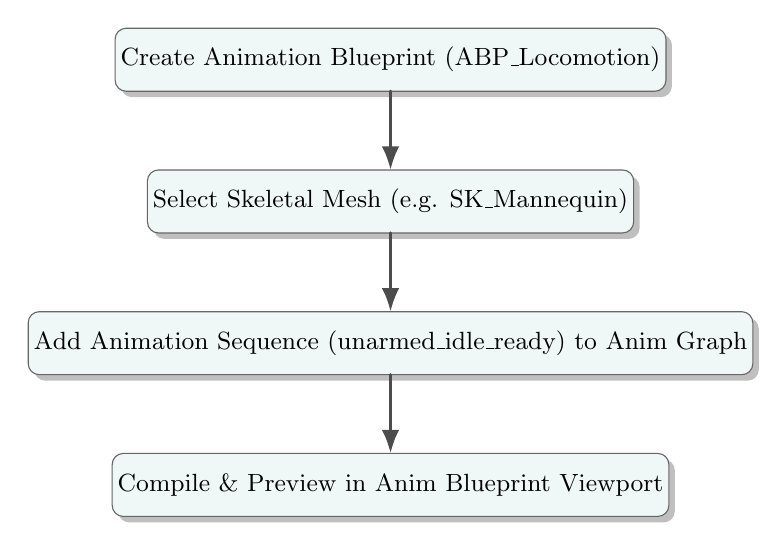
\begin{tikzpicture}[node distance=10mm and 20mm, every node/.style={font=\small}]

  \node[block] (new) {Create Animation Blueprint (ABP\_Locomotion)};
  \node[block, below=of new] (select) {Select Skeletal Mesh (e.g. SK\_Mannequin)};
  \node[block, below=of select] (anim) {Add Animation Sequence (unarmed\_idle\_ready) to Anim Graph};
  \node[block, below=of anim] (preview) {Compile \& Preview in Anim Blueprint Viewport};

  \draw[arrow] (new) -- (select);
  \draw[arrow] (select) -- (anim);
  \draw[arrow] (anim) -- (preview);
\end{tikzpicture}
\end{center}

\subsubsection*{将 Animation Blueprint 分配给角色}
\begin{center}
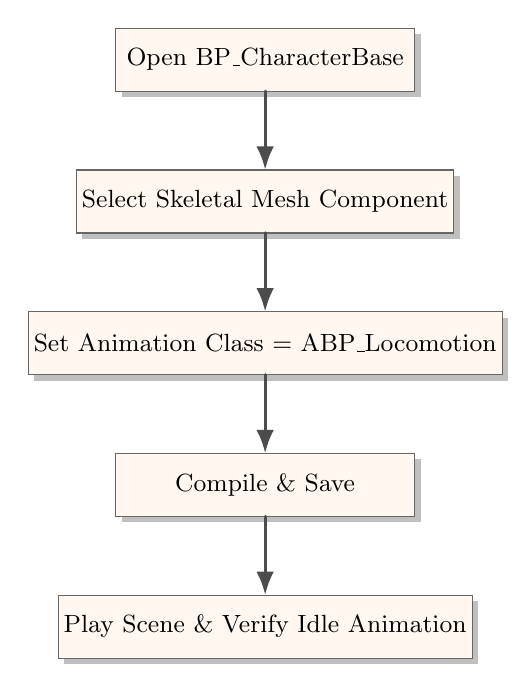
\begin{tikzpicture}[node distance=10mm and 18mm, every node/.style={font=\small}]


  \node[proc] (open) {Open BP\_CharacterBase};
  \node[proc, below=of open] (selectmesh) {Select Skeletal Mesh Component};
  \node[proc, below=of selectmesh] (assign) {Set Animation Class = ABP\_Locomotion};
  \node[proc, below=of assign] (save) {Compile \& Save};
  \node[proc, below=of save] (play) {Play Scene \& Verify Idle Animation};

  \draw[arrow] (open) -- (selectmesh);
  \draw[arrow] (selectmesh) -- (assign);
  \draw[arrow] (assign) -- (save);
  \draw[arrow] (save) -- (play);
\end{tikzpicture}
\end{center}


\subsection{继承影响}
\begin{itemize}
  \item 作者在父级角色类上分配了动画蓝图,因此该更改会自动应用到所有从父类继承的子实例(例如 \il{BP_PlayerBase}、\il{BP_NPCBase}),无需单独为每个子类分配。
  \item 在调试或特殊需求下,可在子类上覆盖父类设置以使用不同的动画蓝图或不同的骨骼网格。
\end{itemize}

\subsection{当前限制与下一步}
\begin{itemize}
  \item 当前仅演示了静态空闲(Idle)动画的绑定与展示;移动时还未播放移动动画(Walk/Run)。
  \item 下一步应:
    \begin{itemize}
      \item 在动画蓝图中添加状态机(Anim State Machine)与参数(例如 Speed、IsMoving),并根据角色的运动状态切换动画(Idle ↔ Walk/Run)。
      \item 将来自角色或角色组件(如 Character Movement)的速度或移动输入传递给动画蓝图(通过变量/接口或直接在蓝图中获取 Pawn 的速度),进而驱动动画过渡。
    \end{itemize}
\end{itemize}

\bigskip
\noindent 小结:本节教会了如何创建动画蓝图、在 Anim Graph 中接入 Animation Sequence、并将 Animation Blueprint 分配给骨骼网格以实现角色空闲动画。后续将实现基于运动数据的动画切换与更复杂的动画逻辑。





\section{状态机与空闲站姿(State Machines and Idle Stance Animation)}

本节说明如何将 Anim Graph 组织为模块化的状态机(State Machine),并通过嵌套状态机与可配置的序列(Sequence)实现可在运行时切换的空闲动画(Idle)。下面给出结构化摘要与关键实现要点。

\subsection{问题陈述}
当前我们只是把空闲动画硬编码接到输出(Result Pose)。随着动画逻辑变复杂(多种空闲、Break 动画、站姿切换等),需要一个模块化、可扩展的设计,以便通过变量/函数在运行时切换动画而无需重复创建多个 Animation Blueprint。

\subsection{总体设计}
核心思路:使用一个顶层的状态机(例如 \il{locomotion}),并在其中嵌套更细粒度的状态机(如 \il{idle} → \il{idleASM} → \il{idleStance}),最终在最内层使用 Sequence Player 播放动画。将具体的 Animation Sequence 暴露为变量(例如 \il{idleAny}),并通过动画节点的回调(如 \il{onUpdate})动态设置该变量,从而实现运行时切换动画。

\subsection{步骤要点}
\begin{enumerate}
  \item 在 Anim Graph 中创建顶层状态机,命名为 \il{locomotion}。
  \item 在 \il{locomotion} 中创建状态 \il{idle},并把 Entry 的默认转换指向该状态(默认状态)。
  \item 在 \il{idle} 状态内部再创建一个状态机(示例名 \il{idleASM}),为后续的空闲子状态(如 \il{idleStance}、\il{idleStart}、\il{idleStop} 等)提供容器。
  \item 在最内层状态(例如 \il{idle})中添加一个 Sequence Player,并将 Sequence 设置为“动态”(promote to dynamic / promote to variable)。
  \item 为该 Sequence 创建一个变量(例如 \il{idleAny}),并将其分类到一个便于管理的 category(如 \il{animSequences})。
  \item 在 Sequence Player 上绑定回调(例如 \il{onUpdate}),并实现一个函数(例如 \il{updateIdleAnimNode}),通过该函数访问 Sequence Player 的节点接口并设置当前播放的 Animation Sequence(带初始融合参数以保证平滑过渡)。
  \item 编译并保存,然后在预览或运行时通过修改 \il{idleAny} 变量观察动画切换效果。
\end{enumerate}

\subsection{关键实现细节与技巧}
\begin{itemize}
  \item 不要把具体序列硬编码在节点上(例如直接把 \il{unarmed_idle_ready} 固定到 Sequence Player),而是把序列作为可配置变量(\il{idleAny})以便不同角色/配置重用同一套 Anim Blueprint。
  \item 将 Sequence Player 转换为可访问的节点(Convert to Sequence Player / PO function),以便在自定义的 \il{onUpdate} 中通过节点输入/输出访问并设置序列与混合时间(blend time,示例 0.2s)。
  \item 在 \il{onUpdate}(或 \il{onBecomeRelevant} / 初始更新)中,通过函数获得对节点的引用并调用设置接口,从而在每帧或首次进入时动态决定播放哪个序列。
  \item 使用合理的命名约定(变量分类、函数分类)可以使蓝图更清晰,例如把所有动画序列变量放到 \il{animSequences} 分类、把动画节点更新函数放到 \il{AnimNod} 或类似分类。
\end{itemize}

\subsection{示意图(嵌套状态机)}
下面给出一个简化的 TikZ 示意图,展示嵌套状态机结构与最终的 Sequence Player:

\begin{center}
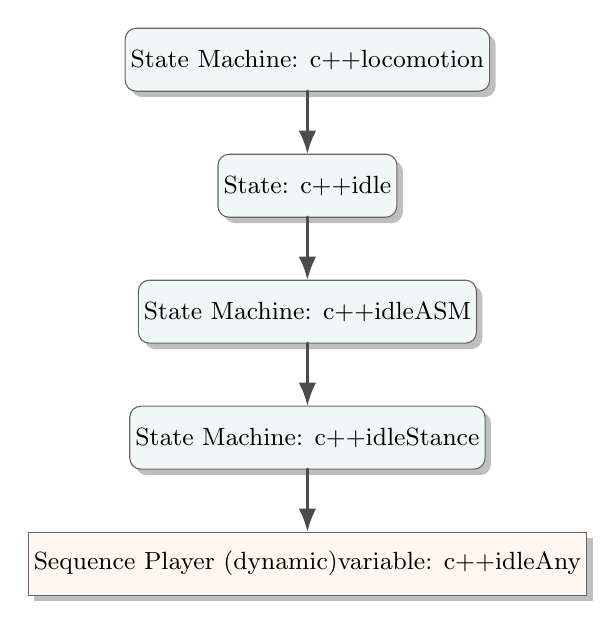
\begin{tikzpicture}[node distance=8mm and 18mm, every node/.style={font=\small}]
  \node[block] (loc) {State Machine: \il{locomotion}};
  \node[block, below=of loc] (idle) {State: \il{idle}};
  \node[block, below=of idle] (idleasm) {State Machine: \il{idleASM}};
  \node[block, below=of idleasm] (stance) {State Machine: \il{idleStance}};
  \node[proc, below=of stance] (seq) {Sequence Player (dynamic) \newline variable: \il{idleAny}};

  \draw[arrow] (loc) -- (idle);
  \draw[arrow] (idle) -- (idleasm);
  \draw[arrow] (idleasm) -- (stance);
  \draw[arrow] (stance) -- (seq);
\end{tikzpicture}
\end{center}

\subsection{运行时演示与验证}
\begin{itemize}
  \item 将 \il{idleAny} 设为某个动画序列(例如 \il{ASMM_unarmed_ready}),编译并保存,预览窗口应播放对应动画。
  \item 通过在编辑器中切换 \il{idleAny} 的值或在运行时由代码/蓝图设置该变量,可以无须修改 Blueprint 代码就切换动画。
  \item 使用初始融合(inertial blending)与短的 blend time(如 0.2s)以提供平滑过渡。
\end{itemize}

\subsection{小结与下一步}
本节将 Anim Graph 组织为多层嵌套状态机,并演示如何把 Sequence Player 参数化为变量,再通过 \il{onUpdate} 类函数在运行时替换播放的动画序列,从而实现复用和模块化的动画系统。下一步可以将状态机扩展以支持 Walk/Run、Turn-in-Place、以及基于速度/方向的 Blend Spaces。\par

\bigskip
\noindent 小结:通过嵌套状态机与可配置的 Sequence Player,可以构建更灵活的空闲动画系统,支持运行时切换与扩展。

\section{Locomotion 系统 Actor Component 与 Animset 数据表(Locomotion System Actor Component and Animset Data Table)}

本节说明如何把动画数据以数据驱动(data-oriented)的方式集中管理,并通过自定义 Actor Component 在运行时将数据注入到动画蓝图,从而实现可扩展的动画配置与切换。下面为结构化摘要与关键步骤。

\subsection{设计目标}
消除在 Animation Blueprint 中的硬编码(例如直接把序列插入节点),把动画资源集中到可编辑的数据表(Data Table)与数据结构(Struct)中,并使用一个可复用的 Actor Component(例如 \il{BPC_Locomotion})在 BeginPlay 或运行时把数据应用到蓝图(变量注入、函数调用)。

\subsection{目录与资源组织}
\begin{itemize}
  \item Blueprints/ActorsComponents/Subsystems:存放子系统用的 Actor Component(例如 \il{BPC_Locomotion})。
  \item Blueprints/Structs/Locomotion:存放动画相关的结构(例如 \il{S_AnimSet})。
  \item DataTables/Locomotion:存放数据表(例如 \il{DT_AnimSet}),每一行对应一个装备/姿态的动画集合(如 Unarmed、Pistol、Rifle)。
\end{itemize}

\subsection{实现步骤(要点)}
\begin{enumerate}
  \item 在蓝图结构(Blueprints → Structures)中创建结构体 \il{S_AnimSet},包含需要的字段(示例:\il{Idle}:Anim Sequence Object Reference)。
  \item 创建数据表 \il{DT_AnimSet},选择行结构为 \il{S_AnimSet},并在表中添加若干记录(Row),例如把一行命名为 \il{Unarmed},并把相应的序列(例如 \il{AS_MM_unarmed_idle_ready})填入 \il{Idle} 字段。
  \item 新建 Actor Component(Blueprint Class → Actor Component),命名为 \il{BPC_Locomotion}(或类似),将其放到 `Actors Components/Subsystems` 下以便归类。
  \item 在父角色蓝图(例如 \il{BP_CharacterBase})中添加该组件实例;Play 时组件会初始化并触发其 BeginPlay(验证方法:在组件中放一个临时的 Print String,如 \il{hello},以确认组件在初始化时被调用)。
  \item 在组件的 BeginPlay 或自定义函数中读取 \il{DT_AnimSet}(通过 Row 名或键),并把读取到的 Anim Sequence 值传递到 Animation Blueprint(例如将动画序列写入 Anim Blueprint 暴露的变量 \il{idleAny},或调用其公开的设置函数)。
  \item 这样一来,切换动画只需在数据表层修改或通过代码/配置选择不同的 Row,无须修改 Animation Blueprint 本体。
\end{enumerate}

\subsection{关键实现细节与建议}
\begin{itemize}
  \item 使用明确的命名规则:结构体使用前缀 \il{S\_}(例如 \il{S_AnimSet}),数据表使用前缀 \il{DT\\_}(例如 \il{DT_AnimSet}),组件使用 \il{BPC\_} 前缀(例如 \il{BPC_Locomotion})。
  \item 在组件中考虑把 Data Table 的引用作为可编辑属性(Editable)暴露在组件 Details 面板,这样设计时可以在各个角色实例中选择不同的表或行。
  \item 读取 Data Table 时,做好空值校验(Row 存在性、字段是否有效),并在缺失时回退到默认动画以避免运行时错误。
  \item 建议在 Data Table 中预留多列(Idle、IdleBreak、Stance、Walk、Run 等),以便后续扩展时只需添加新字段与新记录。
\end{itemize}

\subsection{示意图(数据驱动流程)}
下面给出简化流程图:Data Table 提供动画资源 → Actor Component 读取并在 BeginPlay 注入 → Animation Blueprint 使用这些变量播放动画。

\begin{center}
\begin{tikzpicture}[node distance=10mm and 18mm, every node/.style={font=\footnotesize}]
  % styles
  

  \node[box,font=\footnotesize] (dt) {Data Table: \il{DT_AnimSet} \\\\ (rows: Unarmed, Pistol, ...)};
  \node[box, right=of dt, font=\footnotesize] (comp) {Actor Component: \il{BPC_Locomotion} \\\\ BeginPlay / init};
  \node[box, right=of comp,font=\footnotesize] (abp) {Animation Blueprint: \il{ABP_Locomotion} \\\\ variable: \il{idleAny}};

  \draw[arrow] (dt) -- node[above,font=\footnotesize]{Read row by key} (comp);
  \draw[arrow] (comp) -- node[above,font=\footnotesize]{Inject / Set variable} (abp);
\end{tikzpicture}
\end{center}

\subsection{验证与调试}
\begin{itemize}
  \item 在组件中临时加入日志(Print String),确认 BeginPlay 时组件正确初始化并能读取 Data Table。
  \item 在 Data Table 中切换到另一个 Row(例如从 \il{Unarmed} 切换到 \il{Pistol}),然后运行场景确认对应动画被注入并播放。
  \item 检查空值/类型不匹配,并在组件中提供默认回退行为以保证健壮性。
\end{itemize}

\subsection{小结与下一步}
通过将动画资源集中在结构体与 Data Table 中,并用 Actor Component 在运行时注入这些数据,可以把动画系统变为数据驱动(data-driven)且更易扩展。下一步可实现:在组件层添加配置(例如默认 Row 名、优先级),以及把多个数据源合并(按装备 / 角色类型选择不同的 AnimSet)。

\bigskip
\noindent 小结:数据驱动 + 组件化能把动画设置从 Blueprint 内逻辑中抽离出来,便于跨角色复用与运行时配置。


\section{从数据表获取动画并注入到动画蓝图(Get Animation Data from the Data Table to Animation Blueprint)}

本节演示如何把集中存放在 Data Table 的 AnimSet(例如 \il{DT_AnimSet})读取出来,并通过自定义 Actor Component 将动画序列注入到角色的 Animation Blueprint(Anim BP),实现数据驱动的动画配置与运行时切换。

\subsection{主要目标}
把动画资源与配置从 Animation Blueprint 中抽离出来:
\begin{itemize}
  \item 在组件层公开 Data Table 引用(例如 \il{AnimSetDataTable}),以便在编辑器中为不同角色/实例选择不同的表或记录。
  \item 在组件中提供一个查询函数(例如 \il{GetAnimSet}),给定 Row 名(例如 \il{Unarmed})返回对应的结构化 AnimSet。
  \item 在组件初始化或运行时把读取到的 Anim Sequence 注入到 Animation Blueprint 的暴露变量(例如 \il{idleAny})或调用其公开接口以设置播放动画。
\end{itemize}

\subsection{关键步骤综述}
\begin{enumerate}
  \item 在 `\il{BPC_Locomotion}` 组件中添加一个 public 变量:\il{AnimSetDataTable}(类型:Data Table Object Reference)。
  \item 在组件中实现函数 \il{GetAnimSet}:
    \begin{itemize}
      \item 参数为 Row 名(\il{AnimSetName},类型 Name),并暴露为 public / editable。
      \item 使用 "Get Data Table Row"(或等价节点)读取 \il{AnimSetDataTable},并把结果映射到返回的结构(\il{S_AnimSet})。
      \item 如果找不到 Row,返回空或触发回退逻辑(使用默认 AnimSet)。
    \end{itemize}
  \item 在组件的 BeginPlay(或自定义初始化函数)中:
    \begin{itemize}
      \item 调用 \il{GetAnimSet}(例如默认 Row 为 \il{Unarmed}),取得 Anim Sequence(例如 \il{Idle} 字段)。
      \item 获取拥有该组件的 Pawn / Character(\il{GetOwner} / \il{GetPawnOwner}),再获取其 Skeletal Mesh 的 Anim Instance(\il{GetAnimInstance})。
      \item 将该 Anim Instance 转换(Cast)为你的自定义 Anim Blueprint 类(例如 \il{UABP_Locomotion_C} / Blueprint 的 AnimInstance 类型),或直接调用公开的接口/函数。然后把 Anim Sequence 写入 Anim BP 暴露的变量(例如 \il{idleAny}),或调用类似 \il{SetIdleAnim} 的函数以完成注入。
    \end{itemize}
  \item 编译并在编辑器中验证:在组件 Details 面板中设置 \il{AnimSetDataTable} 为 \il{DT_AnimSet},并把默认 Row 名设置为 \il{Unarmed},运行时应能在 Anim BP 看到对应动画播放。
\end{enumerate}

\subsection{实现提示与鲁棒性}
\begin{itemize}
  \item 在组件层把 DataTable 引用与默认 Row 名设为可编辑(Editable),这样不同角色实例可复用同一组件但指向不同数据。
  \item 在读取 Row 后总是做存在性检查(Row 是否为空、字段是否有效);在失败时使用默认序列或记录日志以便调试。
  \item 使用初始融合(inertial blending)设置序列的 blend time(例如 0.2s)以保证注入时平滑过渡。
  \item 如果想更解耦,可在 Anim BP 中提供一个 BlueprintNativeEvent 或 BlueprintCallable 函数(例如 \il{ApplyAnimSet(AnimSet)}),由组件直接调用该接口而不是直接操作 AnimInstance 字段。
\end{itemize}

\subsection{简化流程图}
\begin{center}
\begin{tikzpicture}[node distance=10mm and 24mm]
  \node[box] (dt) {Data Table: \il{DT_AnimSet}};
  \node[proc, right=of dt] (comp) {Component: \il{BPC_Locomotion} \\\ GetAnimSet / BeginPlay};
  \node[block, right=of comp] (abp) {Anim Blueprint: \il{ABP_Locomotion} \\\ variable: \il{idleAny} / ApplyAnimSet()};

  \draw[arrow] (dt) -- node[above]{Get Data Table Row} (comp);
  \draw[arrow] (comp) -- node[above]{Cast AnimInstance / Call API} (abp);
\end{tikzpicture}
\end{center}

\subsection{小结与下一步}
通过在组件级别读取 Data Table 并把 AnimSet 注入到 Anim BP,可以实现完全数据驱动的动画配置流程。下一步建议:
\begin{itemize}
  \item 扩展 \il{S_AnimSet} 字段以包含更多动作(IdleBreak、Stance、Walk 等)。
  \item 在组件中添加热加载或编辑时回调,以便在编辑器中更改 Data Table 时即时更新 Anim BP(方便迭代)。
  \item 考虑把数据读取逻辑封装为可复用库函数(便于多个子系统调用)。
\end{itemize}

\bigskip
\noindent 小结:本节实现了从数据表读取 AnimSet 并在运行时注入到动画蓝图的流程,提供了可复用、可配置的数据驱动路线。
\end{document}
